\documentclass[12pt]{article}
\usepackage{color}
\usepackage[usenames,dvipsnames,svgnames,table]{xcolor}
\definecolor{dark-red}{rgb}{0.7,0.15,0.15} 
\usepackage[margin=1in]{geometry}
\usepackage[linkcolor=blue,
colorlinks=true,
urlcolor=blue,
pdfstartview={XYZ null null 1.00},
citecolor={blue},
pdftitle={In-N-Out}]{hyperref}
\usepackage[multiple]{footmisc}
\renewcommand{\footnotelayout}{\raggedright}
\usepackage{setspace} 
\usepackage{indentfirst}

\usepackage{verbatim}


\usepackage{titlesec}
\titleformat{\section}{\normalfont \centering}{\thesection}{.5em}{}
\titleformat{\subsection}{\normalfont}{\thesection}{.5em}{}
\setlength{\footnotesep}{0.5cm}

\let\proglang=\texttt
\newcommand{\pkg}[1]{{\fontseries{b}\selectfont #1}}

\newcommand{\superscript}[1]{\ensuremath{^{\textrm{#1}}}}

\usepackage{graphicx}

\usepackage{amsfonts,amssymb,amsbsy}
\usepackage{amsxtra}
\usepackage{amsmath}
\renewcommand{\thefootnote}{\fnsymbol{footnote}}

\usepackage{dcolumn}
\newcolumntype{.}{D{.}{.}{5}}
\newcolumntype{q}{D{.}{.}{3}}
	
\usepackage{natbib}
\bibpunct[, ]{(}{)}{;}{a}{}{,}

\usepackage{amsmath}

\raggedright
\parindent=1.5em % <- or whatever indent you want

\usepackage{caption}


\begin{document}
\doublespacing
\vspace{2cm}

\begin{center}
Explaining Partisan Affect\\Partisans Respond to Partisan Response\\ 
\vspace{2cm}
\today\\\vspace{2cm}

Doug Ahler\footnote{Doug Ahler is Ph.D. candidate in Political Science at the
University of California, Berkeley. Doug can be reached at
\href{mailto:dahler@berkeley.edu}{dahler@berkeley.edu}} and Gaurav
Sood\footnote{Gaurav Sood is a National Fellow at the Hoover Institution at
Stanford University. Gaurav can be reached at
\href{mailto:gsood@stanford.edu}{gsood@stanford.edu}}

\end{center}

\setcounter{page}{0}
\thispagestyle{empty}
\renewcommand*{\thefootnote}{\arabic{footnote}}
\newpage
\setcounter{footnote}{1}


\begin{comment}
	sweaver(paste0(basedir, "xperceive/partisanResponse/manuscript"), "presponse")
\end{comment}
\newpage

Partisans dislike supporters of the opposing party \citep{iyengar2012,
iyengar2013}. Sizable proportions of Democrats and Republicans say they would be
unhappy if a family member of theirs married someone from the opposing party
\citep{iyengar2012}. This widespread mutual antipathy exists despite a vast overlap in policy positions of supporters of both parties \citep{fiorina2012}. If policy differences don't explain this affective gulf, what does?

One potential source of disaffection between partisans concerns not attitudes and opinions themselves but rather perceptions of the validity and thoughtfulness of the other sides' beliefs. Partisans notoriously filter information through a ``perceptual screen'' yielding attitudes and beliefs that prioritize consistency with partisan identity over accuracy and cool reason \citep{TAV,TAVR,Bartels2002}. While the perceptual screen operates largely subconsciously (c.f. Bullock et al. 2013), Democrats observe and lament Republicans' closed-mindedness and vice versa \citep{Haidt2011}.

We start by documenting partisans' tepid reactions to missteps by their own party's elites. We document this using a new database of political scandals, coupled with opinion data from 2000 state level polls measuring approval of Senators, Governors, and the President. We supplement the public opinion data with national panel data from the National Annenberg Election Studies (NAES) and the National Election Studies. We use an interrupted time-series design to measure public opinion before and after political scandals. We find that, indeed, partisans tend not to update evaluations of embattled leaders, which potentially provides fodder for outparty disaffection.

Do perceptions of the outparty as unreasonable and unresponsive to political facts produce enmity between Democrats and Republicans? Answering this question is difficult because partisans very rarely process information about their parties in an unbiased manner, thus yielding few instances in which we can observe how the other side reacts to rank-and-file condemnation of party leaders or policies. Further complicating observational analysis, the rare instances in which party leaders or policies lose significant support among the rank-and-file are likely to be distinct from the usual political kerfuffle that meets with motivated reasoning, rendering comparison between these types of cases sketchy for making causal inferences. 

To avoid these problems and answer this important question, we rely on a randomized, controlled experiment. While Democrats and Republicans rarely update evaluations of party leaders in the face of political snafus in the real world, we use vignettes in which they do to manipulate partisans' sense of intransigence on the other side. By keeping embattled elites and their sources of embattlement constant across treatments and instead manipulating just the degree of change in support among copartisan citizens, we hope to determine whether the perception of reason on the other side affects feelings toward the outparty.

Previewing our results, we find greater affective polarization among partisans exposed to a nonresponse from the outparty to a blunder committed by an outparty elite than among partisans exposed to outparty updating or to a placebo control condition. We further find that strength of partisan identity moderates this effect, with stronger partisans exhibiting greater affective responses to nonresponse among the other side's rank-and-file.

\section*{Study 2: Partisans Respond to Partisan Response}
As the observational data indicate (HOPEFULLY), partisans rarely update their evaluations of their parties' leaders in the wake of scandals and political errors. Observational data can, thus, only take us so far, as we lack a counterfactual for identifying the effect of perceived outparty intransigence on affect toward the outparty. To solve this problem, we randomly assign respondents to read about differing partisan responses to party elites' political errors. 

\subsection*{Research Design}
In November 2013, we recruited 930 survey participants through Amazon'sMechanical Turk \citep[see][]{BerinskyHuberLenz2012}. We randomly assigned participants to read a news story on one of three ongoing political scandals at the time: the troubled rollout of the U.S. health exchange website (Democratic Party blunder), Ted Cruz's inflammatory rhetoric precluding compromise during the shutdown and debt ceiling negotiations (Republican Party blunder), and Toronto mayor Rob Ford's drug scandal (placebo control condition). Within news stories on American party leaders' political errors, we randomly assigned participants to one of two conditions related to partisan reaction. In one condition (``response''), participants read that support for the embattled elite (President Obama or Cruz) declined among co-partisan citizens. In the other condition, (``no response''), participants read that support for the elite remained steadily high. See Appendix A for a complete transcript of the stories.

We assessed whether exposure to stories in which partisans withdraw support from their party's elites when they learn about the political scandal, compared to both the control condition and the condition in which partisans continue to support their leaders despite the political scandal, changed evaluations of the rank-and-file of the party whose elite was embroiled in the scandal. In particular, after exposing respondents to the stories, we asked the respondents how well they thought each of eight traits---ignorant, sincere, open to reason, smug, selfish, patriotic, compassionate, and hypocritical---described ``people who support the Democratic (Republican) Party'' on a semantic five-point scale, ranging from ``extremely well'' to ``not at all.'' We recoded ratings on negatively-valenced traits so that all trait ratings ranged from negative to positive. We next created a difference score as a summary measure of partisan affect (The $\alpha$ for difference ratings was .90).

To test the hypothesis that an effect would be moderated by respondents' degree of party identification, political interest, and political knowledge, we also measured these concepts. Party identification was measured using the conventional branched question found in the ANES. Political interest was self-reported, while knowledge was measured with five questions about civics and current events. (See SI section XX for these specific items.)

\section*{Analyses and Results}

Before random assignment to experimental conditions, we measured whether or not the respondents were paying attention to the survey. In particular, we posed a question that asked respondents to mark two particular responses. Of the 930 respondents, 38 respondents failed to complete the task as requested. We removed these participants from our sample as we felt that they were merely adding noise to the data.

Given our theory and the nature of the intervention, we further limit ourselves to analyzing responses from supporters of the two major parties (including leaners). This limits our respondent pool to $n=726$.

The Mechanical Turk community heavily overrepresents Democrats. 552 of the 726 respondents (over 75\%) either leaned towards the
Democratic party or identified as Democrats outright. In the interest of clarity but also in line with where most of our data lies, we first start by analyzing Democratic responses. Furthermore, since our theory engages how partisans react to outparty supporters' responses to their elites' missteps, we analyze data from the control, `Republicans--Change,' and `Republicans--No Change' conditions.

As Figure 1 shows, Democratic respondents assigned to the `Republicans--No Change' condition report greater antipathy toward
Republicans, as measured by differenced average trait ratings (b = .06, $p < .11$, see Table 1). These respondents further report more polarized evaluations of the parties than Democrats assigned to the `Republicans--Change' condition (b = .07, $p < .06$). However, Democrats exposed to the story that Republicans updated their evaluations of Senator Cruz in the wake of the shutdown did not report evaluations of Republicans that were significantly different from those of control participants. 

\begin{figure}
\caption{Evaluative Polarization Between Experimental Conditions (Democratic Respondents)}
\begin{center}
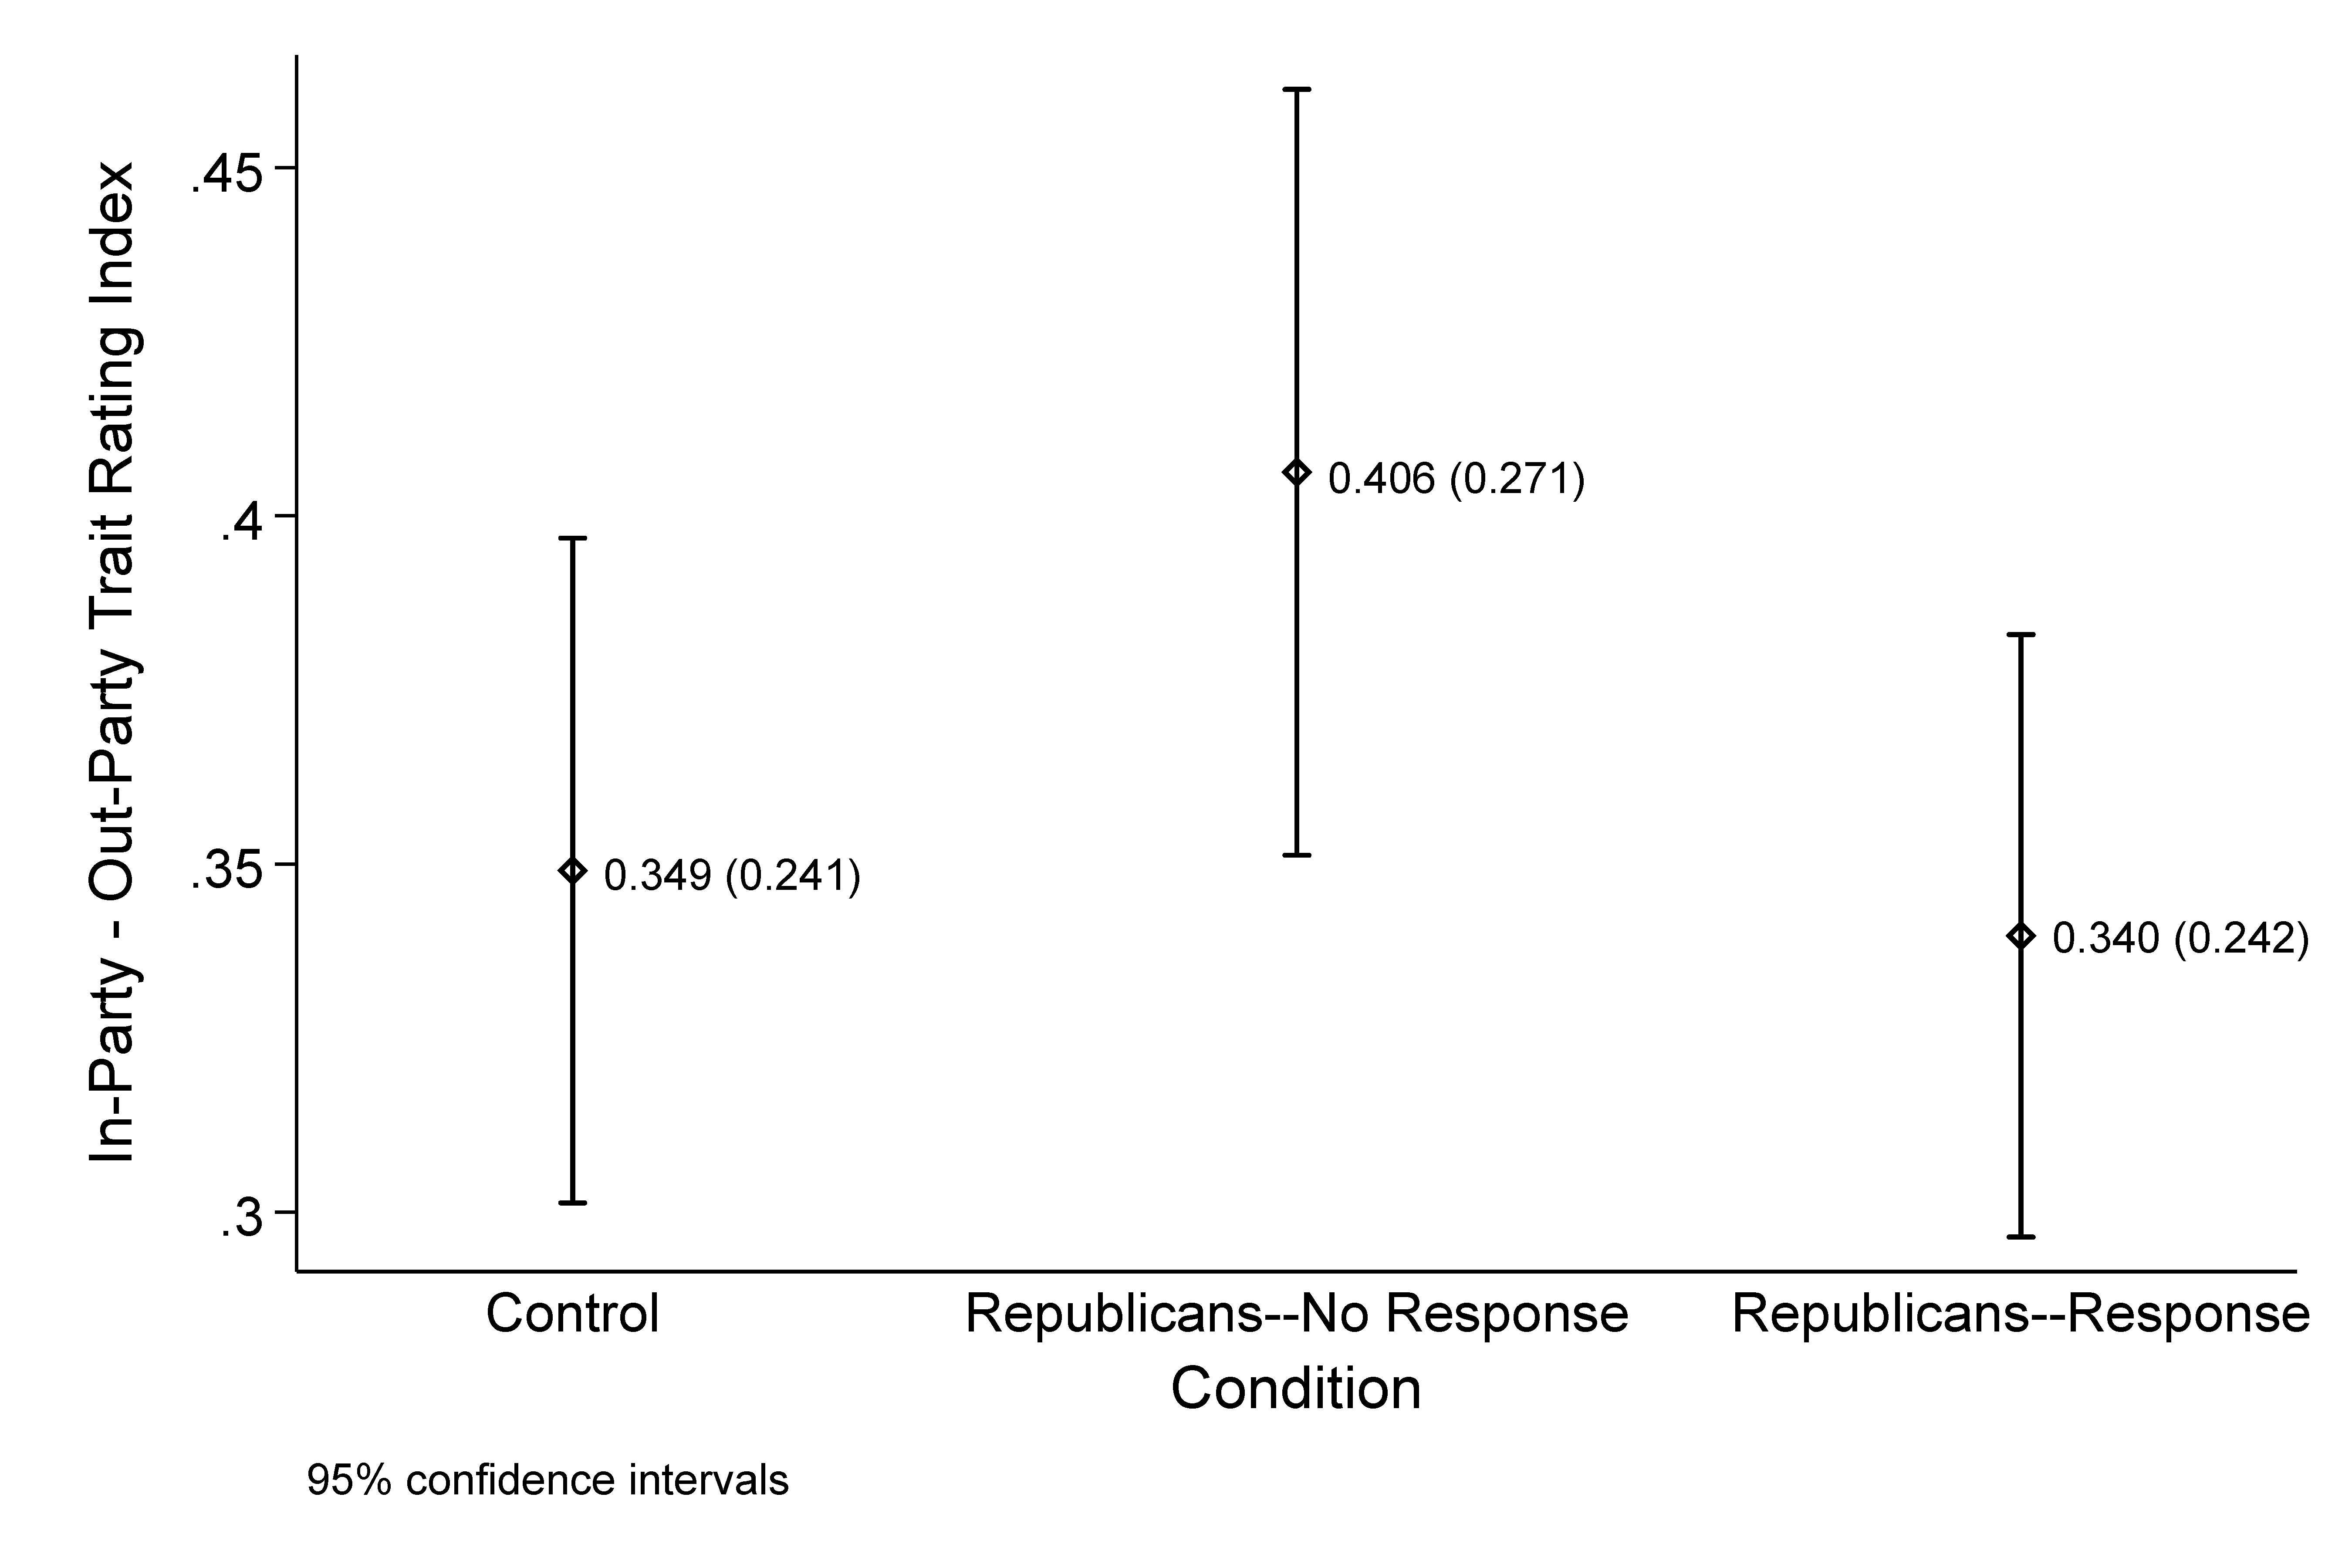
\includegraphics[scale=0.3]{ciplot_dems_on_reps.pdf}
\end{center}
\end{figure}

\centerline{(Insert Table 1 here.)}

As hypothesized, strength of party identification moderates this apparent effect. As Table 2 shows, strong Democrats assigned to both the control condition (column 1) and the `Republicans--Response' condition (column 2) demonstrate greater polarization in their evaluations of the two parties, indicating that strength of party identification is associated with greater evaluative bias. However, this tendency becomes more pronounced in the `Republicans--No Response' condition. The interaction of strength of partisan identification and assignment to the `Republicans--No Response' condition is substantively and statistically significant, indicating that strong Democrats react more vehemently to learning that their Republican peers failed to change their attitudes toward Ted Cruz in the wake of the government shutdown. 

\centerline{(Insert Table 2 here.)}


\clearpage
\singlespacing
\nocite{BullockEtAl2013}

\bibliographystyle{apsr_fs}
\bibliography{xperceive}  

\clearpage 
\section*{Tables}
<<echo=F, results=tex, label=setup>>=
# Loading Functions
	source(paste0(basedir, "func/func.R"))

# Load libraries
	library(xtable)
	library(apsrtable)
	#library(lattice)
	#library(gridExtra)
	
# Load experiment data
		pr <- read.csv(paste0(basedir, "xperceive/PartisanResponse/data/pr.recode.csv"))

		
# Cronbach's alpha for diff. in ratings
	# a <- zero1(cbind(pr$rep_traits_1r, pr$rep_traits_2r, pr$rep_traits_3r, pr$rep_traits_6r, pr$rep_traits_8r)) - 	#	zero1(cbind(pr$dem_traits_1r, pr$dem_traits_3r, pr$dem_traits_3r, pr$dem_traits_6r, pr$dem_traits_8r))
	# ltm::cronbach.alpha(a,standardized = FALSE, CI = FALSE, probs = c(0.025, 0.975), B = 1000, na.rm = TRUE)$alpha	

	# Eliminate inattentive
		# Proportion inattentive small. interesting. we need to eliminate that check up front.
		pr <- subset(pr, attentive)
	
		
	
	# Eliminate Independents
		pr <- subset(pr, pid3!='Independent')
	
	# Only Democrats are worth investigating for now
	# Subsets
		# R conditions + control
			prc <- subset(pr, pid3=='Democrat' & treat %in% c("Control", "R Change", "R No Change"))
		# R conditions
			prr <- subset(pr, pid3=='Democrat' & !is.na(ronly))
		# D conditions
			prd <- subset(pr, pid3=='Democrat' & !is.na(donly))
		
	# Basic Analyses
		r0only  <- with(pr[pr$pid3=='Democrat',], lm(rdtrt ~ treat))
		r1only	<- with(prc, lm(rdtrt	~ treat))
		r2only	<- with(prr, lm(rdtrt	~ treat))
		
		apsrtable(r0only, r1only, r2only, model.names=c("R-D Trt", "R-D Trt", "R-D Trt"), caption="Within Democrats")
	
	# Interactions
		r1only	<- with(prc[prc$pid7 < 3,], lm(rdtrt	~ treat))
		r2only  <- with(prc[prc$pid7 < 2,], lm(rdtrt	~ treat))
		r3only	<- with(prc[prc$know > 0,], lm(rdtrt	~ treat))

		apsrtable(r1only, r2only, r3only, model.names=c("Str./Weak Dems.", "Strong Dems.", "Know > 0"), caption="Within Democrats")
		
	# Basic Analyses with diff. trait battery
			r1only	<- with(prr, lm(reptrt2	~ treat))
			r2only	<- with(prr, lm(rdtrt2	~ treat))
			r3only	<- with(prr, lm(rdtrt2	~ treat*pid7))
				
		apsrtable(r1only, r2only, r3only, model.names=c("Rep Trt", "R-D Trt", "R-D Trt with Pid7"), caption="Within Democrats")
		
	# Manipulation check data...
		
@
\clearpage
\singlespacing
<<echo=T>>=
	# Traits: Mean and Median 
	with(pr[pr$pid3=='Democrat',], aggregate(rdtrt, list(treat), mean, na.rm=T))
	with(pr[pr$pid3=='Democrat',], aggregate(rdtrt, list(treat), median, na.rm=T))
@
\clearpage
\section*{Appendix A}


\begin{figure}[ht]
\centering
\begin{minipage}[b][12cm][b]{0.45\linewidth}
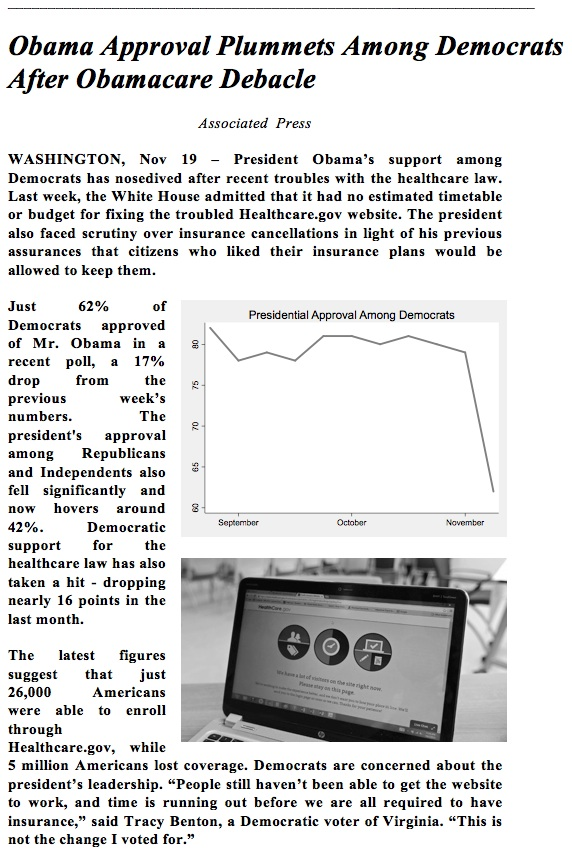
\includegraphics[width=1.05\textwidth]{../Manipulations/Dem_C.jpg}
\caption{Democrats Withdraw Support}
\label{fig:minipage1}
\end{minipage}
\quad
\begin{minipage}[b]{0.45\linewidth}
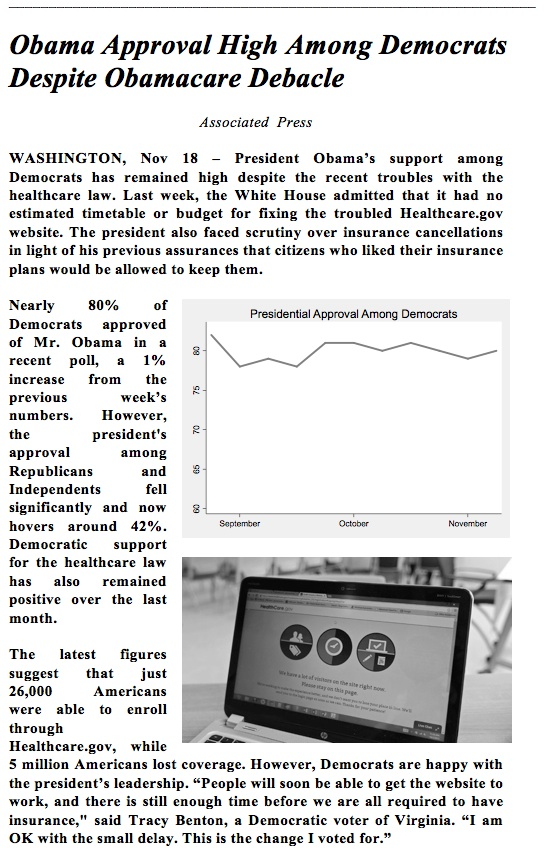
\includegraphics[width=1\textwidth]{../Manipulations/Dem_T.jpg}
\caption{Democrats Continue Support}
\label{fig:minipage2}
\end{minipage}
\end{figure}

\begin{figure}[ht]
\centering
\begin{minipage}[b][12cm][b]{0.45\linewidth}
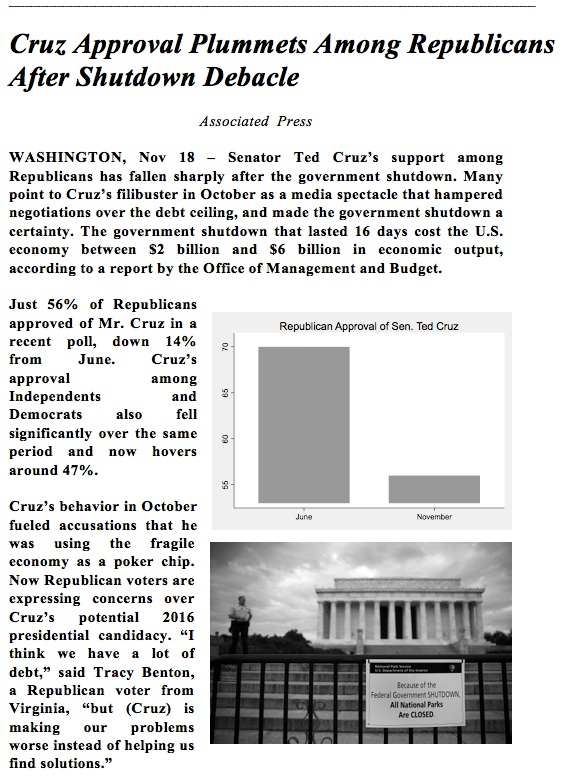
\includegraphics[width=1.05\textwidth]{../Manipulations/Rep_C.jpg}
\caption{Republicans Withdraw Support}
\label{fig:minipage3}
\end{minipage}
\quad
\begin{minipage}[b]{0.45\linewidth}
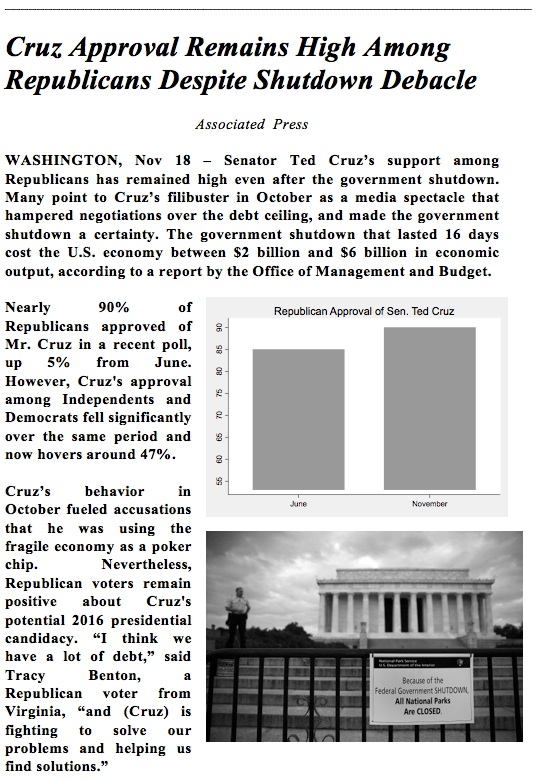
\includegraphics[width=1\textwidth]{../Manipulations/Rep_T.jpg}
\caption{Republicans Continue Support}
\label{fig:minipage4}
\end{minipage}
\end{figure}

\end{document}